% IEEE standard conference template; to be used with:
%   spconf.sty  - LaTeX style file, and
%   IEEEbib.bst - IEEE bibliography style file.
% --------------------------------------------------------------------------

\documentclass[letterpaper]{article}
\usepackage{spconf,amsmath,amssymb,graphicx}
\usepackage{graphicx}
\usepackage{tabularx}
\usepackage[export]{adjustbox}


% Example definitions.
% --------------------
% nice symbols for real and complex numbers
\newcommand{\R}[0]{\mathbb{R}}
\newcommand{\C}[0]{\mathbb{C}}

% bold paragraph titles
\newcommand{\mypar}[1]{{\bf #1.}}

% Title.
% ------
\title{Parallel SAT Solving}
%
% Single address.
% ---------------
\name{Jan Eberhardt, Jakub Lichman}
\address{Department of Computer Science\\ ETH Zurich\\Zurich, Switzerland}

% For example:
% ------------
%\address{School\\
%		 Department\\
%		 Address}
%
% Two addresses (uncomment and modify for two-address case).
% ----------------------------------------------------------
%\twoauthors
%  {A. Author-one, B. Author-two\sthanks{Thanks to XYZ agency for funding.}}
%		 {School A-B\\
%		 Department A-B\\
%		 Address A-B}
%  {C. Author-three, D. Author-four\sthanks{The fourth author performed the work
%		 while at ...}}
%		 {School C-D\\
%		 Department C-D\\
%		 Address C-D}
%

\begin{document}
%\ninept
%
\maketitle
%

The hard page limit is 6 pages in this style. Do not reduce font size
or use other tricks to squeeze. This pdf is formatted in the American letter format, so the spacing may look a bit strange when printed out.

\begin{abstract}
Describe in concise words what you do, why you do it (not necessarily
in this order), and the main result.  The abstract has to be
self-contained and readable for a person in the general area. You
should write the abstract last.
\end{abstract}

\section{Introduction}\label{sec:intro}

\mypar{Motivation} Boolean satisfiability problem (SAT) belongs to the most important problems in program analysis, verification and other disciplines of theoretical computer science. It is particularly used in background of many applications, especially ones in the field of automated planning and scheduling, model checking(formal verification) and theorem proving. 

Last decade brought many improvements to SAT world in form of advanced heuristics, preprocessing and inprocessing techniques and data structures that allow efficient implementation of search space pruning. 

However, past 10 years were also rich on improvements in parallelism. Current trends in computer hardware design decreased performance per processing unit and pack more units on a single processor. It is caused by thermal wall which stopped further increase of clock speed. However, algorithms for SAT solving like DPLL and CDCL were invented before wide use of parallelism and therefore were designed for sequential execution. Since SAT is a NP-complete problem, we consider it the right candidate for running in parallel.

In our approach, we are trying to speed up SAT solving by running it on multiple cores with different techniques of search space partitioning. Final comparison is done between different parallel versions and sequential one. Parallel versions are mainly based on DPLL algorithm except the one which uses also CDCL, but locally. All algorithms are unlimited in number of cores they can run on. However, some scale better than the others. 

Experiments were run on the cluster where we were allowed to use at most 48 cores. Tests were taken from SATLIB - The Satisfiability Library \cite{cnf_website} and some were also created by our own random generator of formulas. Results show nice speedups in parallel versions against sequential one. However, parallel DPLL algorithm is still not able to outperform sequential CDCL. It shows how good CDCL actually is in comparison with DPLL. 

\mypar{Related work} Tomas Balyo et al. in their paper \cite{hordesat} propose HordeSat solver which can run up to 1024 cores and is based on CDCL algorithm. Their parallel approach is different from ours because it is portfolio based but with sign of search space partitioning. Most of the previous SAT solvers designed for computer clusters or grids use explicit search space partitioning. Examples of such solvers are GridSAT \cite{gridsat}, PMSAT \cite{pmsat} or ManySat \cite{manysat}. Paper that is probably closest to ours \cite{stealing} firstly introduced work stealing for dynamic load-balancing. 

\section{Background: Whatever the Background is}\label{sec:background}

\mypar{CNF} A \textit{boolean variable} is a variable that can be assigned either to \textit{true} or \textit{false}. A \textit{literal} of a boolean variable $x$ is considered to be in positive $x$ or negative  $\overline{x}$ form. A \textit{clause} is then disjunction (OR) of literals. A \textit{conjunctive normal form} (CNF) is a conjunction of such a clauses. CNF is usually represented by a number of variables and clauses.  However, measuring difficulty of CNF by these two factors is very inaccurate.  

\mypar{SAT} SAT solver is a program that is able to decide whether given formula is satisfiable. More formally, given formula $F$ is satisfiable \textit{iff} there \textit{exists} assignment of literals $\theta$ that makes whole formula (\textit{CNF}) true (\textit{satisfiable}). If there does not exits such an assignment then formula is \textit{unsatisfiable}. Furthermore, every SAT solver should be able in \textit{satisfiable} case provide valid assignments of literals as well. 

\mypar{History} First algorithm was develop in 1960 by Martin Davis and Hilary Putnam \cite{dp} for checking the validity of a first-order logic formula using a resolution-based decision procedure for propositional logic. Since Davis-Putnam algorithm was able to handle just valid formulas, more general approach for SAT solving was needed. In 1962 was developed new, complete algorithm that was able to handle all types of formulas. The algorithm is called \textit{DPLL} \cite{dpll} after Davis, Putnam, Logemann, and Loveland. It is backtracking-based search algorithm that still forms the basis for most efficient complete SAT solvers. Since DPLL invention, there were many algorithms proposed, which improved runtime of SAT solving significantly.
\begin{figure}
	\centering
	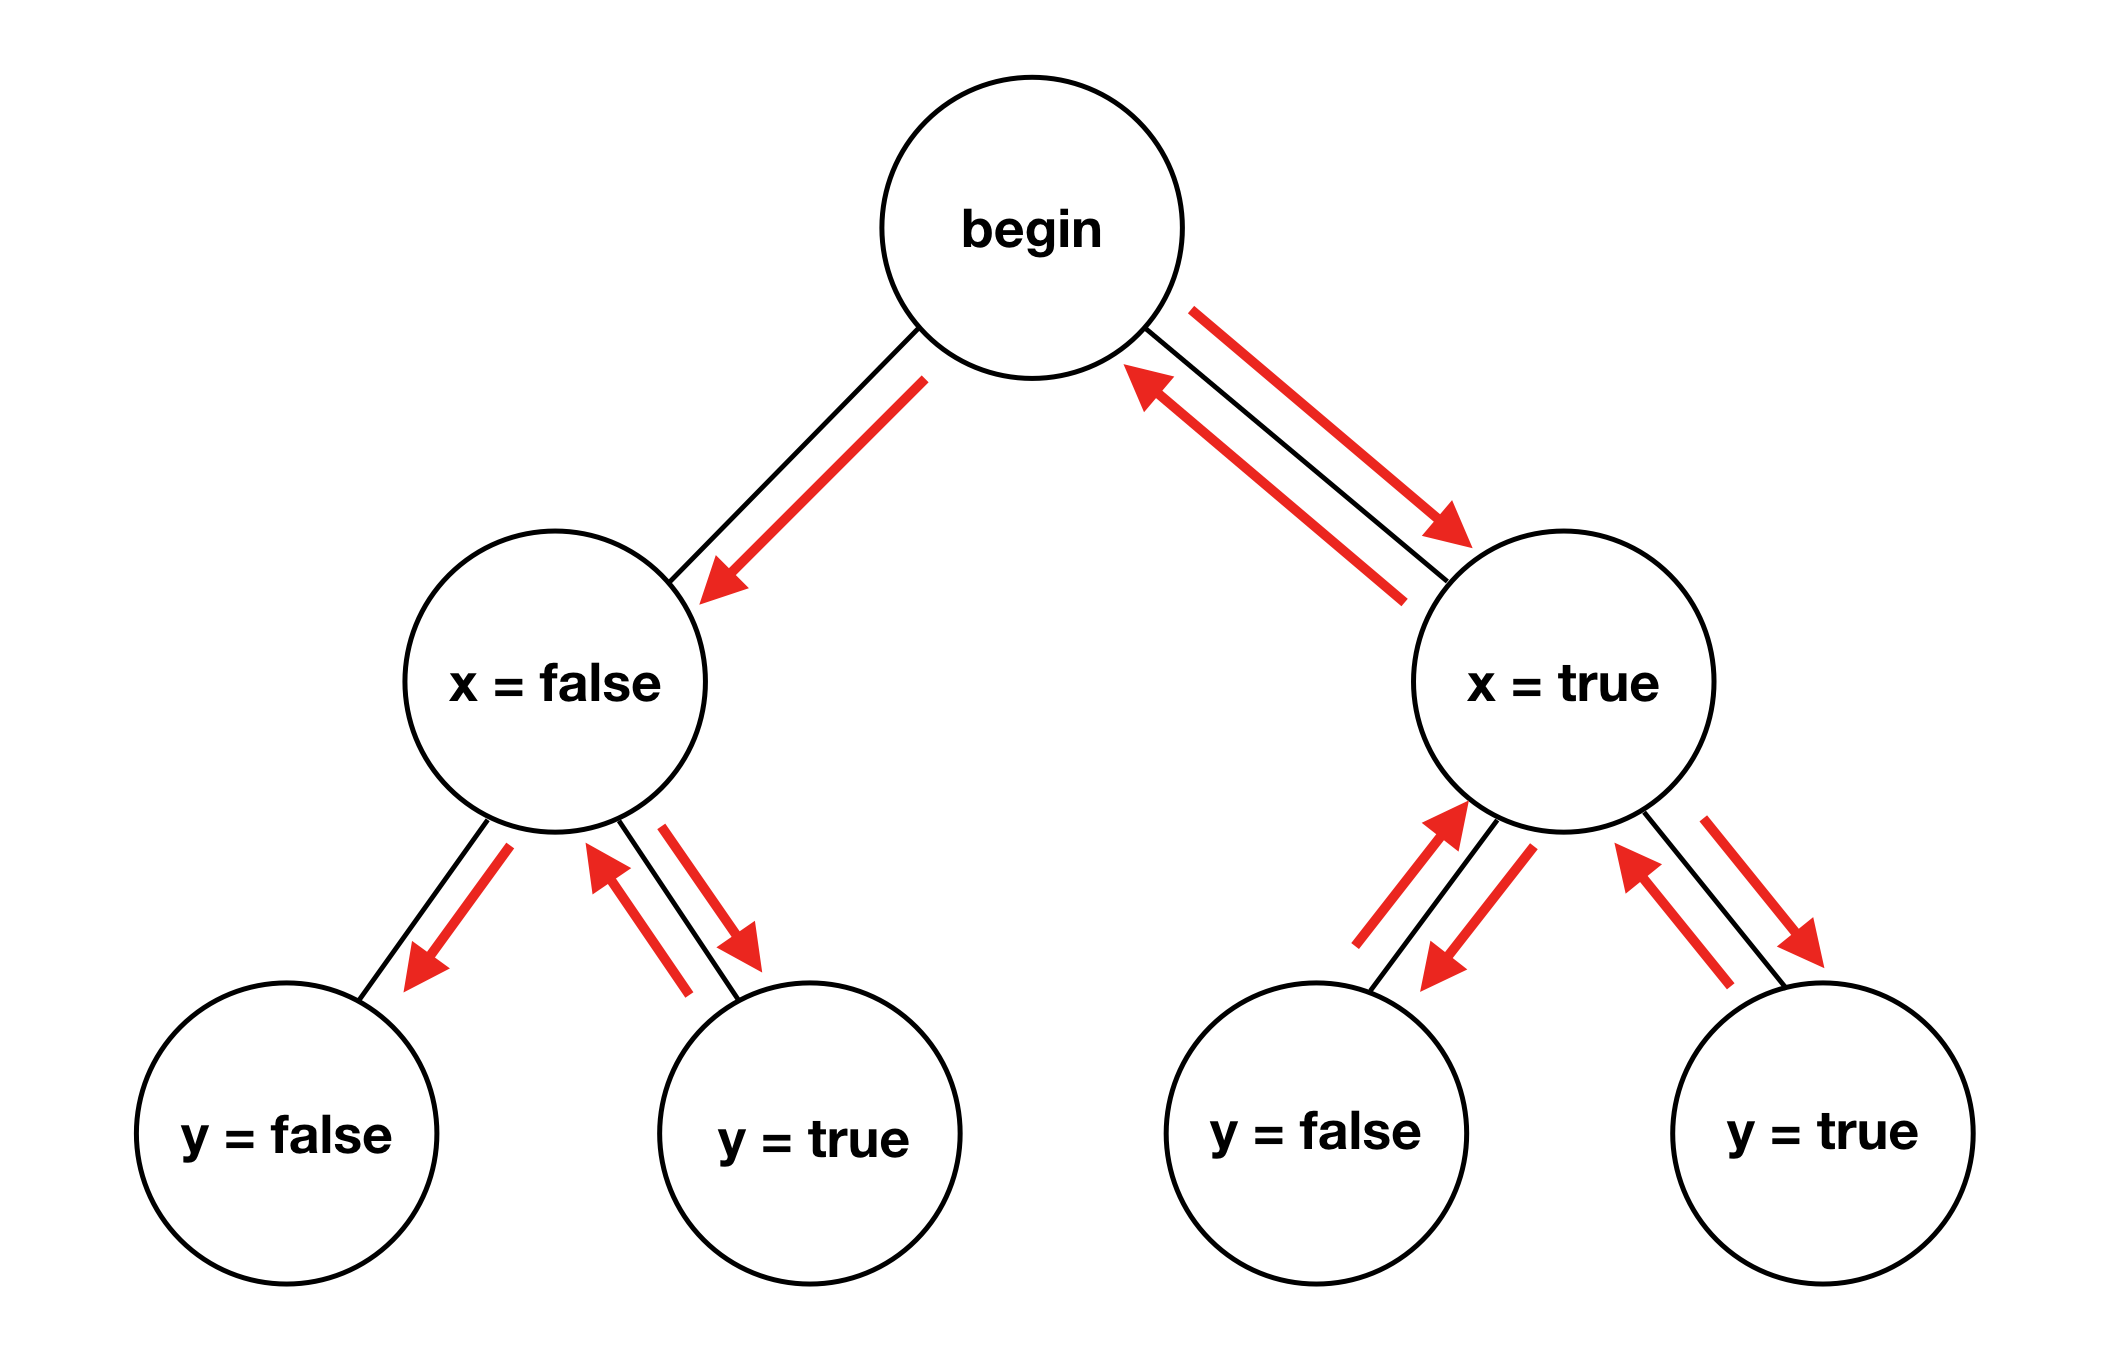
\includegraphics[width=\columnwidth]{figures/dpll-branching}
	\caption{The way how DPLL explores search space of CNF with two variables \textit{x} and \textit{y}.
		\label{fig:dpll-branching}}
\end{figure}

\mypar{DPLL} DPLL solves a SAT problem by modelling it as a decision tree, variables can either be assigned to \textit{true} or \textit{false}. In every step DPLL tries to find variables that are "automatically" assigned because of a previous decision,
if there are none it will pick a variable $v_i$ and assume a value for it.
If it later turns out that this decision was wrong it backtracks to that point and picks the negated assignment for variable $v_i$.

\mypar{CDCL} The algorithm performs as well as DPLL a depth-first search of the space of partial truth assignments. In addition to DPLL, Conflict-Driven Clause Learning (\textit{CDCL}) adopts a pruning technique called learning. While in DPLL we can solve same clauses multiple times, CDCL remembers them and in the next encounter avoids them. More formally, learning extracts and memorizes information from the previously searched space to prune the search in the future \cite{cdcl}. Learning is done by adding clauses to the existing clause database. Clauses are analyzed and stored whenever search reaches conflict state. If it cannot be resolved by backtracking then the formula is unsatisfiable. If all the variables are assigned and no conflict happened then the formula is satisfiable. \cite{hordesat}


\section{Parallelizing DPLL}\label{sec:parallel_dpll}

DPLL is a simple backtracking algorithm that explores search space without any advanced techniques like learning and pruning. As an result of this, it does not require any transfer of information between stages of solving and therefore it can be nicely parallelized. Parallelization is not trivial but far easier than in case of CDCL where in addition to load balancing we need to deal with learned clause sharing. 

%We decided to parallelize DPLL because it is a relatively simple backtracking algorithm and therefore it does not require any advanced communication. Subtasks can be solved individually and therefore also on different nodes.

\mypar{DPLL Branches}
As shown in figure \ref{fig:dpll-branching} the DPLL algorithm explores search space with depth first search. However it needs to make a decision at some point. If there are no more literals that can be assigned trivially, we need to pick the one and assume it to be either \textit{true} or \textit{false}. That is exactly the point where we can do so called DPLL branching, i.e. let some other node solve the other branch. We can call this point branching point and it represents one node in DPLL search space graph. 

In our work we considered two approaches to load balancing. 
%We looked at two different ways on how to split the work between multiple nodes. 
First one is a master worker communication pattern, where one node called \textit{master} is in charge of storing partial models and eventually passing them to \textit{workers} that will solve them.
Second approach is a work stealing communication model where each node (\textit{worker}) runs on its own and therefore all \textit{workers} are equal. If some \textit{worker} runs out of work and the formula is not solved yet, it picks a random other \textit{worker} and tries to steal partial model from it.

\mypar{Master Worker Model}
First approach that we have decided to design and implement is master worker model. We considered this model to be easiest to implement and therefore we picked it first. The biggest challenge in parallelizing DPLL is load balancing. The work cannot be split equally between workers at the beginning because it would require knowledge of a depth of each branch that cannot be inferred from a formula at the beginning. We want to avoid situations where work is not divided equally because we want to fully exploit computing power of all nodes. 

Master is one of \textit{n} nodes available and other \textit{n-1} nodes become \textit{workers}. At the beginning are all workers marked as free. Master starts solving model by passing empty model to the first free worker. Each worker in every branching point takes one branch and sends the other to the master. When master receives partial model, it checks whether there exists some free worker. If not then it stores the model into its local stack and sends it back in case some worker finished its branch with \textit{unsat} and therefore needs more work. If there is still some free worker then master bypasses the partial model to it. This procedure is repeated until some worker does not find \textit{sat} model and sends it to the master. Master then outputs the model and stops all workers. If no worker found \textit{sat} model, master has empty stack and all workers are free we know that formula is \textit{unsat}.

While master worker model is easy to understand and implement it comes with several drawbacks. First of them is lack of one node. Master worker model has one node used only as an manager and therefore this node is not actually doing any computation. Next issue is related to scaling. Master with certain number of nodes becomes bottleneck because there is too much communication it needs to process and therefore nodes need to wait longer for getting new model. Last problem is related to amount of communication in this model. There is transfer of models and meta data every time worker branches or wants to get a new model. There is also transfer at the beginning and at the end but this communication is necessary while the one mentioned before can be reduced.  

\mypar{Work Stealing Model} Because of the drawbacks mentioned above we have decided to reduce and decentralize communication by implementing work stealing model which provides desired features. The model treats all nodes \textit{equally} and therefore there is \textit{no master} just workers. All workers contain their own stacks with models to process. This reduces communication overhead because all produced models are stored locally instead of their transfer and storage on the master. However, existence of local stack breaks load balancing because some workers can work on bigger subtrees of search space than the others.

Inequalities in load balancing are resolved by mechanism called work stealing. In case some worker finished its work and no other worker has solved the formula than it tries to "steal" model from other workers. Process of stealing can be formally defined as follows: Try to steal from random worker until you do not find a model or until someone else has not find it. We need to define two more rules(phases) for algorithm to work. First phase is initial work distribution and second one is ending condition. In initial phase worker 0 will take role of the master and distribute starting models to all workers. Then will all workers try to solve their subtrees and in case of running out of work they will do stealing (phase 2). When some worker will find a \textit{sat} model then it will send it to the worker 0 and it will stop all workers and output final assignment (phase 3). We have to have master node at the end because there can be more workers that find \textit{sat} model at the same time. In our solution, worker 0 prints first obtained sat model and ignores the others.

However, our current work stealing implementation has one drawback. It can only handle satisfiable cases. The stopping criteria in the unsatisfiable case was very trivial in master worker model because it was moment when master's stack was empty and all workers were free. In work stealing no such a moment exits. We do not have central node that controls the others and therefore knows in which stage each worker is. We currently cannot detect if all workers are trying to steal (no worker has work left) and therefore we restrict ourselves just to sat formulas but we plan to solve this issue in our future work. 

\mypar{Implementation}
We implemented both communication models in C++ with a help of the MPI \cite{mpi}.
Our DPLL solver is implemented in C++ as well and therefore we can directly interact with MPI within the solver. We tried to keep implementation of a DPLL algorithm and communication within a nodes as separate as possible for better readability.
The implementation of a parallel DPLL is straight forward and tries to follow good object oriented programming principles. We adapted test driven development with python wrapper that tests our program as black box. We split program into classes with well defined interfaces according to their functions and applied proper encapsulation and information hiding. 

We used \textit{vector}s from the C++ standard library to represent sets of clauses and sets of literals. We used \textit{unsigned int}s as variable names, and \textit{boolean} types for sign, literal and variable values. 
%values for sign and value of the literal and variable.
To implement the backtracking algorithm we used recursion, but we allocate all necessary data structures on the heap.
We didn't experience any stack overflow issues.

\mypar{Correctness}
We tested our sequential DPLL solver on hundreds of formulas that we either randomly generated or took over from a SATLIB formula collection. \cite{cnf_website}
We ran each formula through z3 \cite{z3} and compared the result of the z3 with our result.
The following cases have to be considered for each test case:
\begin{itemize}
    \item If both solvers return unsat, we pass the test case.
    \item If one solver returns sat and the other one unsat, we fail the test case.
    \item If both solvers return sat, we still need to check if the model our solver has returned is correct.
        To do that we can conjoin the model to the original formula and again run it through z3.
\end{itemize}

We ran the both parallel implementations through the same set of formulas and checked correctness for each of them.
Assuming that our sequential implementation is correct, it is straight forward that our parallel implementation is correct as well, since we essentially solved the same set of subproblems but on the different nodes and in completely different order. The difference between parallel and stealing version is in load balancing and not in searched space, i.e. both versions solve the same partial models but they are distributed over working nodes in a different way.


\section{Experimental Results}\label{sec:exp}
In this section we are going to present our experimental results for both versions of our parallel DPLL algorithm as well as their detailed description.

\mypar{Experimental Setup}
We ran both communication models on the Euler super compute cluster \cite{euler} on up to 48 cores, which was the maximum accessible number of cores to us, and requested 1 Gigabyte of memory per core. Euler contains 5 different types of nodes but each of them contains at least two 12-core Intel Xeon processors (2.5-3.7 GHz) and between 64 and 512 GB of DDR4 memory clocked at 1866, 2133 or 2666 MHz.

\mypar{Benchmark Formulas} During our correctness testing and debugging phase of the core algorithm, we realized that random formulas generated by our own random formula generator are not suitable for performance testing. Even if we picked formulas that contained the same amount of variables, clauses and literals per clause, we observed the variation of runtimes between them. It is caused by a completely random structure of a formula generated by our generator. Therefore we used a set of 14 formulas taken from the SATLIB as a benchmark set.
The set contains different real world problems modeled as a boolean formulas from various domains such as planning problems, all-interval series encodings, flat graph coloring, inductive inference, etc. Our benchmark set also contains few random formulas that were taken from SATLIB as well. 
Table \ref{tab:benchmark_set} in the Appendix section contains a detailed listing of the used formulas together with their description. For the coming subsections we reduced the set of benchmark formulas to a representable subset of size 6 for readability reasons and included corresponding figures for the other 8 formulas in the Appendix section. Subset of representatives is described in table \ref{tab:cnfs_representatives}.

\mypar{Master Worker}
We compared the runtimes of the master worker communication pattern with the sequential version of the DPLL. The achieved speedup is shown in Figure \ref{fig:dpll_parallel_speedup}.
\begin{figure}
    \centering
    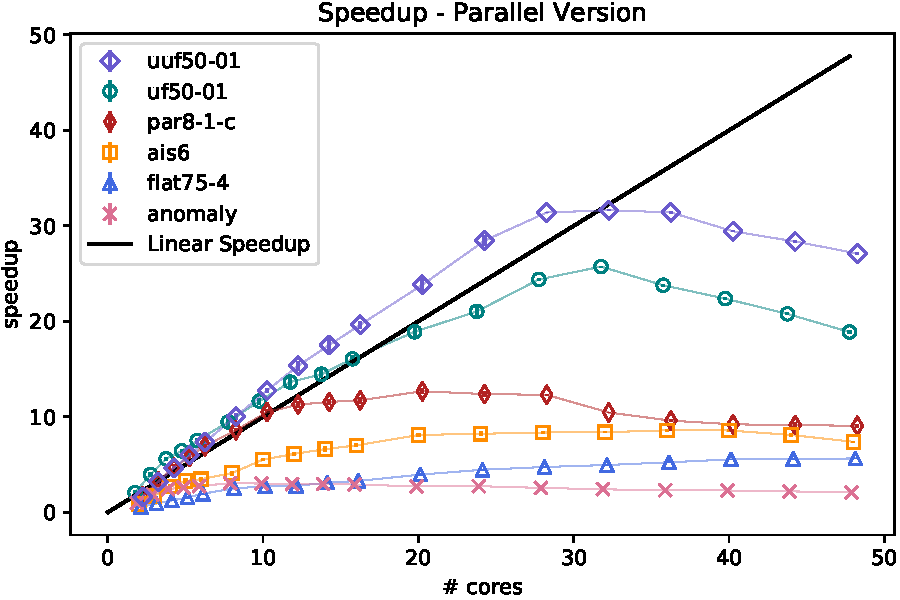
\includegraphics[width=\columnwidth]{figures/scaling_parallel_subset_dpll_scaling_tar.pdf}
    \caption{Average speedup of master worker parallel DPLL implementation compared to sequential DPLL.
    The 95\% confidence intervalls are shown as error bars but too small to be visible in some cases.
    \label{fig:dpll_parallel_speedup}}
\end{figure}
It can be inferred from the figure that achieved speedup factor heavily depends on the formula.
However size of the problem together with the time required to solve a formula with the sequential algorithm are not the only influential factors. 
%original: But it is not just the "size" of the problem or time required to solve a formula with the sequential algorithm that influences the speedup factor.
As shown in Table \ref{tab:cnfs_representatives} the formulas where we reached the highest speedup are not necessarily the ones with the longest time to solve sequentially or the largest number of variables (highest upper bound on the depth of the decision tree).
Note that the best speedup in this subset is achieved with the randomly generated formula (uf50-01).
For these types of formulas it is trivial to explain why speedup goes down with more than 32 cores.
It is caused by moments in solving process when master is no longer able to serve that many workers at the same time and therefore some workers has to wait longer for obtaining next partial model. This problem starts to occur when number of cores overcome 30. 
Another graph that shows this problem is the overall average waiting time shown in Figure \ref{fig:dpll_parallel_waiting}.
Waiting time in our paper is considered to be time that some worker spends waiting for new partial model from master.
The overall waiting time is then sum of all waiting time periods over all workers and then averaged over different runs of the same formula.

The cases where speedup is not so significant are real world problems and therefore their decision trees have some structures. The small speedup is then caused by the way a decision tree is traversed.
While the sequential implementation deterministically does a depth-first search and therefore gives us ordering guarantees, parallel version sends all subbranches to a master and gives no guarantees that it will receive them in the next call to a master. 
It might happen that we are "close" to a solution but then we receive partial model in a completely different part of the decision tree that might be unsatisfiable all together. 
The size of the subtree where we will not find a solution depends on the structure of the formula.
This is also the explanation why we achieved super linear speedup in some other cases. There we were lucky enough in traversing the decision tree and because of that we found a solution faster than in the sequential traversal.

\begin{table}
    \centering
    \begin{tabular}{|l|c|c|}
        \hline
        Formula & runtime seq. DPLL [ms] & \# vars/clauses \\
        \hline
        \hline
        uf50-01 (sat) & 7890.9 $\pm$ 44.31 & 50/218\\
        \hline
        par8-1-c (sat) & 2185.0 $\pm$ 32.88 & 64/254\\
        \hline
        ais6 (sat) &  2964.0 $\pm$ 41.54 & 61/581\\
        \hline
        flat75-4 (sat) & 26284.6 $\pm$ 172.65 & 225/840\\
        \hline
        anomaly (sat) & 279.7 $\pm$ 6.74 & 48/261\\
        \hline
        uuf50-01 (unsat) & 13404.2 $\pm$ 102.94 & 50/218\\
        \hline
    \end{tabular}
    \caption{Overview of benchmark subset formulas.}
    \label{tab:cnfs_representatives}
\end{table}

\begin{figure}
    \centering
    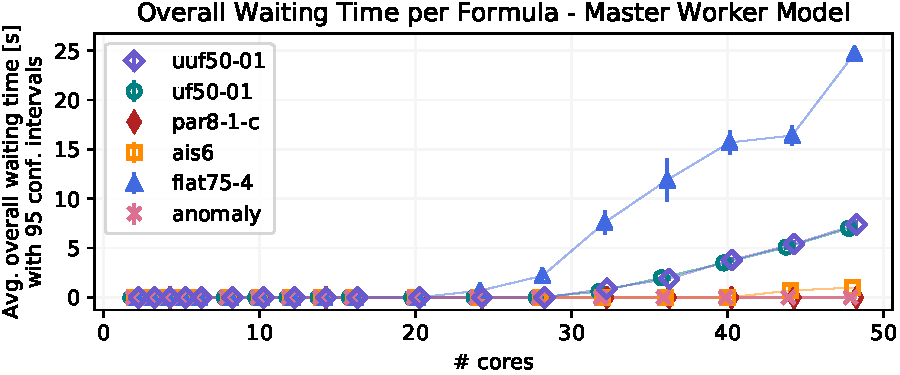
\includegraphics[width=\columnwidth]{figures/waiting_parallel_subset_dpll_scaling_tar.pdf}
    \caption{Average overall waiting time of workers per cnf in parallel version.
    All waiting times per worker are summed up.
    The 95\% confidence interval are shown as error bars.}
    \label{fig:dpll_parallel_waiting}
\end{figure}

\mypar{Work Stealing}
Similar to the previous comparison, we compared the parallel work stealing algorithm to the sequential version of the DPLL.
\begin{figure}
  \centering
  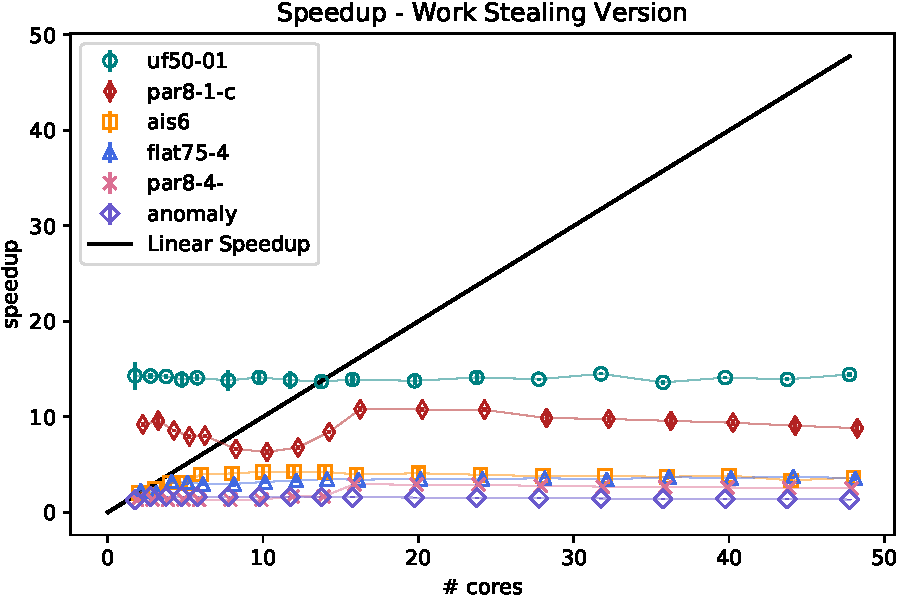
\includegraphics[width=\columnwidth]{figures/scaling_stealing_subset_dpll_scaling_tar.pdf}
  \caption{Speedup of work stealing parallel DPLL implementation compared to sequential DPLL.
  \label{fig:dpll_stealing_speedup}}
\end{figure}

The speedup that we achieved is shown in Figure \ref{fig:dpll_stealing_speedup}.
With work stealing pattern we achieved super high speedups for small numbers of cores but essentially did not gain from adding more cores after some limit.
The reason for this speedup is again the way how we traverse the decision tree.
In this pattern we do something that is similar to a breath first search globally and locally per node, the traversal order of the subtree is the same as in the sequential implementation, so depth first search.
That means that if the formula is satisfiable, we are guaranteed that some worker is working on the correct subtree already after the first decision and will never solve models of the other, wrong subtree.
This guarantee we do not have for the master worker pattern and we therefore beat the master worker pattern easily.

\section{Discussion}
In this section we will mention some of the things that we tried along the way but did not work out or we had to stop looking closer into because of time constraints.

\mypar{CDCL DPLL Hybrid Parallel Solver}
We have implemented a fully working CDCL solver.
If run sequentially it outperforms the DPLL solver on all of our 14 benchmark formulas.
Quite naturally we tried to plug that solver in at the workers.
The way we did that is the following:
\begin{itemize}
    \item First we run DPLL in parallel (it does not matter which of two communication patterns we pick).
    We only branch a certain number of times per worker.
    \item After that "branching limit" is reached we switch to CDCL and solve the whole subtree of the original decision tree locally.
    \item When that is done we either found a solution or again get a new model (either from the master or another worker) and solve it with CDCL.
\end{itemize}
With this hybrid approach we achieved really bad performance.
There are two reasons why.
Firstly we essentially cripple the CDCL solver by not giving him the full formula but only modified a part of it.
That means if we already decided something and then pass on that subproblem to the CDCL solver, the subproblem has not really a correlation to the original problem.
The problem that we solve with CDCL can be a completely different one and therefore a lot more difficult to solve then the original one.
Secondly, yet again we break something because of the way we split the work:
It might happen that all workers are busy solving some problem that is a lot more difficult than the actual problem and the subproblem that contains the correct solution is not solved by any worker at that point in time.
That means in the worst case we solve lots of partial models that are more difficult than the original problem, before we solve the correct problem and find the solution.

We ran everything we discussed in Section \ref{sec:exp} with this hybrid parallel solver for different branching limits.
We do not include any further information in this report because of space limitations.

\section{Future Work}
In this section we discuss possible extensions of our work.

\section{Conclusions}

Here you need to summarize what you did and why this is
important. {\em Do not take the abstract} and put it in the past
tense. Remember, now the reader has (hopefully) read the report, so it
is a very different situation from the abstract. Try to highlight
important results and say the things you really want to get across
such as high-level statements (e.g., we believe that .... is the right
approach to .... Even though we only considered x, the
.... technique should be applicable ....) You can also formulate next
steps if you want. Be brief. After the conclusions there are only the references.

% References should be produced using the bibtex program from suitable
% BiBTeX files (here: bibl_conf). The IEEEbib.bst bibliography
% style file from IEEE produces unsorted bibliography list.
% -------------------------------------------------------------------------
\bibliographystyle{IEEEbib}
\bibliography{bibl_conf}

\newpage
\section{Appendix}
This section contains additional information that is not strictly part of the report.

\begin{table}[h]
    \centering
    \begin{tabularx}{\columnwidth}{|l|X|}
        \hline
        File names & Description\\
        \hline
        \hline
        anomaly, medium & SAT-encoded blocks world planning problems\\
        \hline
        ais6, ais8 & SAT-encoded All-Interval Series problems\\
        \hline
        flat50-1, flat75-4 \\ flat 75-8 & SAT-encoded "Flat" Graph coloring problems (J. Coberson's flat graph generator is used\\
        \hline
        ii8a1 & Inductive inference, stem from a formulation of boolean function synthesis problems\\
        \hline
        par8-1-c, par8-4- & Instances for learning the paritiy function\\
        \hline
        uf50-01, uf75-01 & Uniform random 3-sat, satisfiable\\
        \hline
        uuf50-01, uf50-02 & Uniform random 3-sat, unsatisfiable\\
        \hline
    \end{tabularx}
    \caption{Description of benchmark problems.}
    \label{tab:benchmark_set}
\end{table}

\begin{figure}[h]
    \centering
    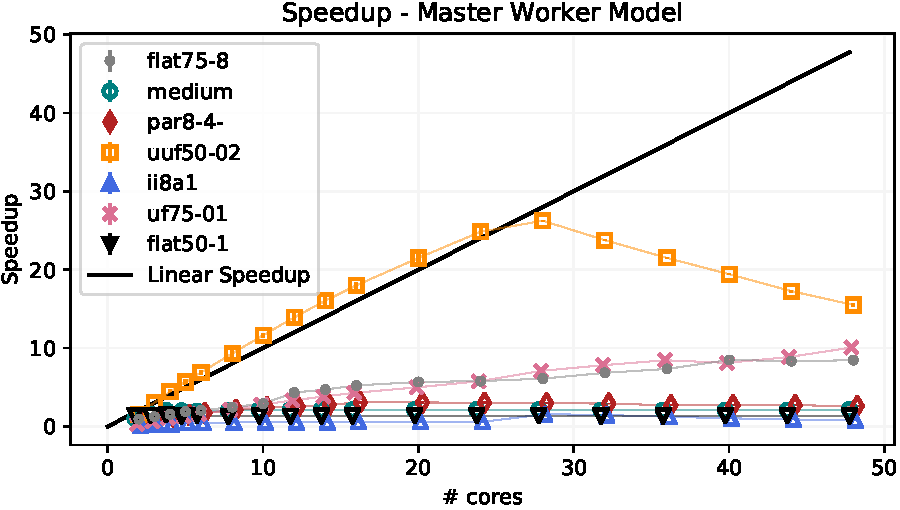
\includegraphics[width=\columnwidth]{figures/scaling_parallel_non_subset_dpll_scaling_tar.pdf}
    \caption{Average speedup of master worker parallel DPLL implementation compared to sequential DPLL.
    The 95\% confidence intervalls are shown as error bars but too small to be visible in some cases.
    Other subset.}
    \label{fig:dpll_parallel_speedup_non}
\end{figure}

\begin{figure}[h]
    \centering
    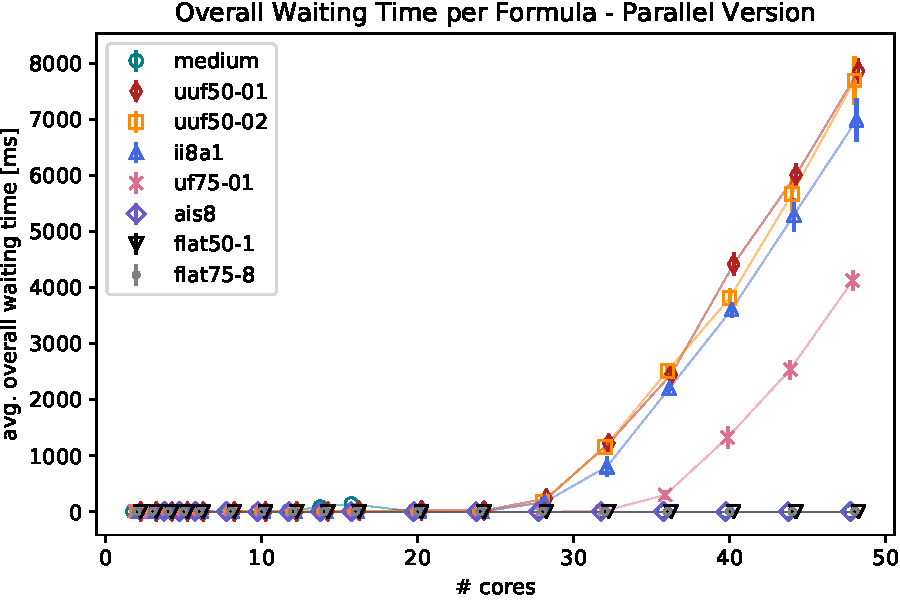
\includegraphics[width=\columnwidth]{figures/waiting_parallel_non_subset_dpll_scaling_tar.pdf}
    \caption{Average overall waiting time of workers per cnf in parallel version.
    All waiting times per worker are summed up.
    The 95\% confidence interval are shown as error bars.
    Other subset.}
    \label{fig:dpll_parallel_waiting_non}
\end{figure}

\begin{figure}[h]
    \centering
    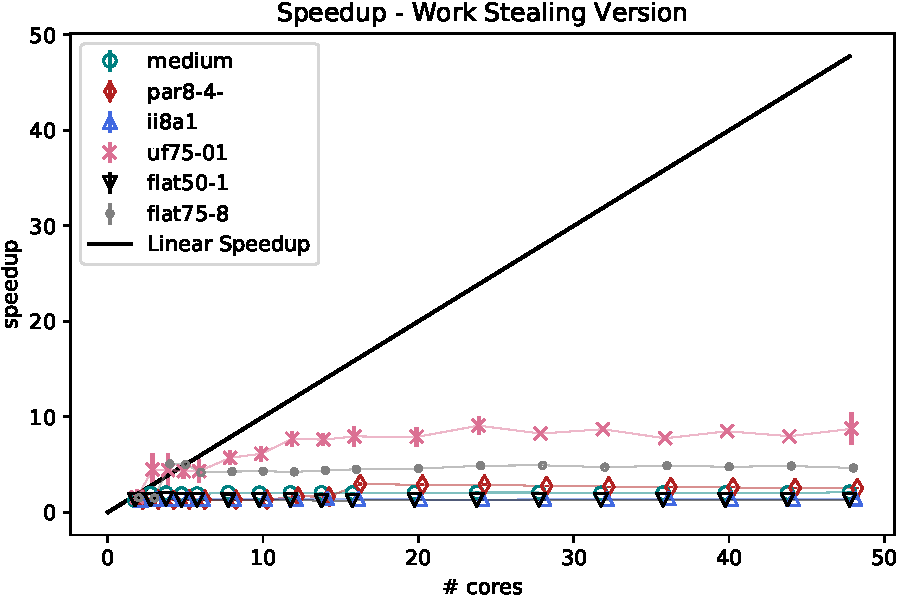
\includegraphics[width=\columnwidth]{figures/scaling_stealing_non_subset_dpll_scaling_tar.pdf}
    \caption{Speedup of work stealing parallel DPLL implementation compared to sequential DPLL.
    Other subset.}
    \label{fig:dpll_stealing_speedup_non}
\end{figure}

\begin{figure}[h]
    \centering
    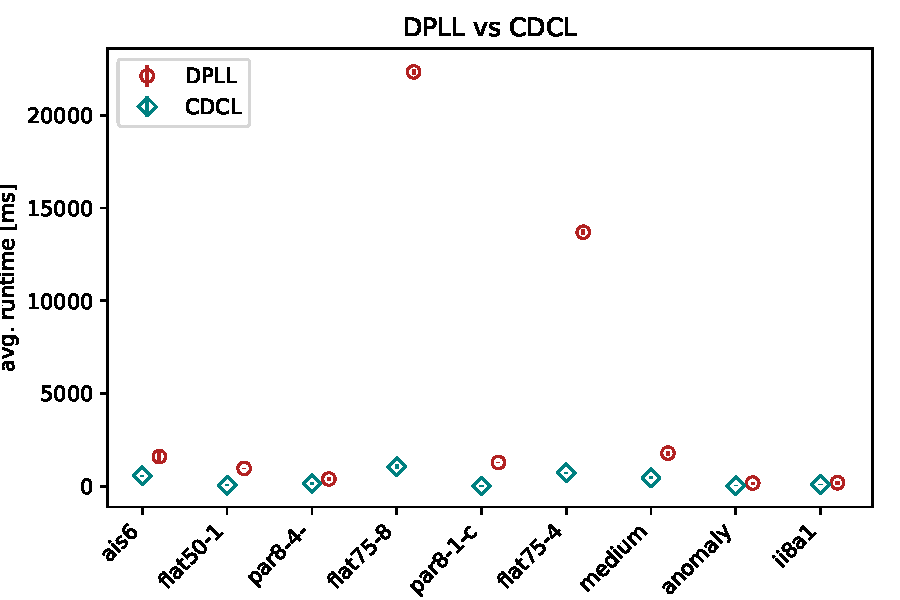
\includegraphics[width=\columnwidth]{figures/dpll_vs_cdcl.pdf}
    \caption{DPLL vs CDCL sequential runtime. Average runtime with 95\% confidence intervals.}
    \label{fig:dpll_stealing_speedup_non}
\end{figure}

\begin{table}
    \centering
    \begin{tabular}{|l|l|c|}
        \hline
        Formula & Best Solver Configuration & Runtime [ms]\\
        \hline
        \hline
        anomaly & CDCL sequential & 16.2 $\pm$ 4.18 \\
        \hline
        medium & CDCL sequential & 414.8 $\pm$ 32.94 \\
        \hline
        ais6 & DPLL master worker, 14 cores & 343.3 $\pm$ 3.58 \\
        \hline
        ais8 & DPLL master worker, 48 cores & 3015.3 $\pm$ 58.85 \\
        \hline
        flat50-1 & CDCL sequential & 36.4 $\pm$ 9.07 \\
        \hline
        flat75-4 & CDCL sequential & 702.8 $\pm$ 38.18 \\
        \hline
        flat75-8 & CDCL sequential & 1054.2 $\pm$ 50.72 \\
        \hline
        ii8a1 & DPLL master worker, 6 cores & 72.2 $\pm$ 0.79 \\
        \hline
        par8-1-c & CDCL sequential & 15.2 $\pm$ 2.28 \\
        \hline
        par8-4- & DPLL master salve, 2 cores & 132.2 $\pm$ 2.22 \\
        \hline
        uf50-01 & CDCL sequential & 31.5 $\pm$ 9.21 \\
        \hline
        uf75-01 & DPLL master worker, 32 nodes & 297.4 $\pm$ 7.99 \\
        \hline
        uuf50-01 & DPLL master worker 24 nodes & 187.5 $\pm$ 5.59 \\
        \hline
        uuf50-02 & DPLL master worker 24 nodes & 148.9 $\pm$ 2.85 \\
        \hline
    \end{tabular}
    \caption{Benchmark formulas with best performing configuration.}
    \label{tab:cnfs_parallel}
\end{table}


\end{document}

